\newlength{\bibsep}
\documentclass[nonatbib,5p,a4paper]{elsarticle}
\usepackage[english]{babel}
\usepackage[DatePublished]{code/style}
\usepackage{csquotes}
\usepackage{lipsum}
\usepackage{amsmath}
\usepackage{cuted}
\usepackage{derivative}
\selectlanguage{english}

\let\oldsqrt\sqrt
% it defines the new \sqrt in terms of the old one
\def\sqrt{\mathpalette\DHLhksqrt}
\def\DHLhksqrt#1#2{%
\setbox0=\hbox{$#1\oldsqrt{#2\,}$}\dimen0=\ht0
\advance\dimen0-0.2\ht0
\setbox2=\hbox{\vrule height\ht0 depth -\dimen0}%
{\box0\lower0.4pt\box2}}

\makeatletter
\newcommand*{\overrightharpoonup}{\mathpalette{\overarrow@\rightharpoonupfill@}}
\newcommand*{\rightharpoonupfill@}{\arrowfill@\relbar\relbar\rightharpoonup}
\makeatother

\DeclareFontFamily{U}{matha}{\hyphenchar\font45}
\DeclareFontShape{U}{matha}{m}{n}{
      <5> <6> <7> <8> <9> <10> gen * matha
      <10.95> matha10 <12> <14.4> <17.28> <20.74> <24.88> matha12
      }{}
\DeclareSymbolFont{matha}{U}{matha}{m}{n}
\DeclareMathSymbol{\varrightharpoonup}{3}{matha}{"E1}
\let\rightharpoonup\varrightharpoonup
\newcommand*{\vect}{\overrightharpoonup}

\addbibresource{bibliography/sources.bib}

\begin{document}

\begin{frontmatter}

\title{%
\textbf{Factors Affecting the Damping Constant of a Spring System}\\
\small Submitted for assessment in 12A\_PHY1
}

\author{James Bray} 
\address{Christ Church Grammar School}

\newdate{dateName}{2}{09}{2025} % edit the date here, ' dateName ' has to match on these two lines.
\renewcommand*{\today}{\DayMonthYearDateFormat\displaydate{dateName}} 

\NameOfAbstract{Abstract}
\begin{abstract}

\lipsum[0-1]

\end{abstract}

\end{frontmatter}
\begin{figure}
    \centering
    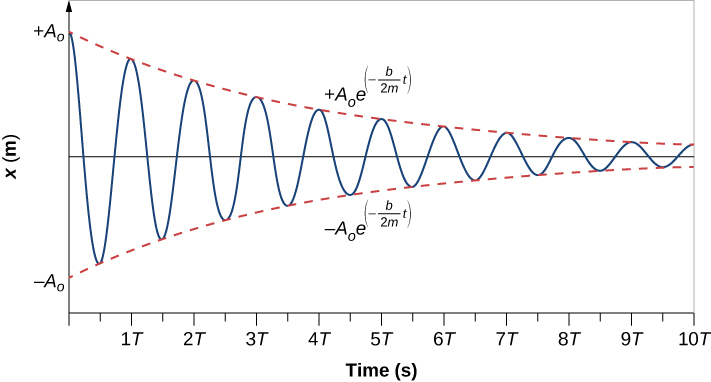
\includegraphics[width=0.47\textwidth]{images/damped_shm.png}
    \caption{Displacement--time graph illustrating the characteristics of an underdamped harmonic oscillator.}
\end{figure}

\section{Introduction}

A vertical mass--spring system provides a simple model for studying oscillatory motion and energy dissipation in mechanical systems. An ideal mass--spring system undergoes simple harmonic motion with constant amplitude, but in real conditions mechanical energy is dissipated through a variety of means, causing oscillations to gradually decrease in amplitude. This phenomenon is known as damping, defined as "the loss of energy of an oscillating system by dissipation."

The degree of damping can be characterised by the decay constant $\gamma$, which specifies the rate at which oscillations diminish; larger values correspond to faster energy loss and more rapid amplitude reduction. The value of this constant depends on both the properties of the oscillating mass and the restoring system.

\subsection{Aim and Hypothesis}
The aim of this investigation is to determine how spring configuration and attached mass influence the rate of damping, quantified by the exponential decay constant $\gamma$, in a vertically oscillating mass-spring system.

It is hypothesised that if the attached mass is increased, there will be a decrease in the decay constant $\gamma$ proportional to $m{\textsubscript{load}}^{-1}$, and if the spring system is configured in series, there will also be a decrease in the decay constant.

The primary sources of damping are expected to be internal friction within the spring in conjunction with resistive forces such as air drag on the mass. For simplicity, it will be assumed that these factors can be modelled by a damping force which is linearly dependent on velocity, as with a standard viscous dampening model.

\subsection{Variables}
\begin{description}
    \item[{\small\bfseries Independent Variables:}] The mass of the load attached to the end of the spring, and the configuration of the spring system.
    \item[{\small\bfseries Dependent Variable:}] The curve-fitting coefficients of the damped harmonic motion displacement-time graph.
    \item[{\small\bfseries Controlled Variables:}] The positioning of the retort stand and clamps, motion sensor alignment and sampling frequency, mass cross-sectional geometry, and ambient air conditions (temperature, pressure, humidity).
\end{description}
\clearpage
\section{Theory}

\lipsum[30-36]
\section{Method and Equipment}

\lipsum[4-5]

\section{Results}

\lipsum[5-6]

\setlength{\tabcolsep}{4pt} % default ~6pt
\begin{table}[!ht]
	\caption{Regression parameters for the light spring.}
    \centering
    \begin{tabular}{|
        S[table-format=1.5,table-number-alignment=center] !{\vrule width 1.2pt}
        S[table-format=1.5] |
        S[table-format=1.5] |
        S[table-format=1.2] !{\vrule width 1.2pt}
        S[table-format=1.4] |
    }
    \hline
    \rowcolor{lightgray}
    {$m{\textsubscript{load}}$} & {$A$} & {$\gamma$} & {$\omega'$} & {$R^2$}\\
    \rowcolor{lightgray}
    {(\si{\kilo\gram})} & {(\si{\meter})} & {(\si{\per\second})} & {(\si{\radian\per\second})} & {}\\
    \hline
    0,05025 & 0,01133 & 0,02424 & 21,47 & 0,9990 \\
	0,10014 & 0,01220 & 0,01752 & 15,43 & 0,8385 \\
	0,15044 & 0,02408 & 0,01478 & 12,53 & 0,9947 \\
	0,20011 & 0,04302 & 0,01326 & 10,89 & 0,9996 \\
	0,25019 & 0,04420 & 0,01224 & 9,75 & 0,9894 \\
	0,30012 & 0,11210 & 0,01183 & 8,92 & 0,9999 \\
	0,34991 & 0,13050 & 0,01138 & 8,28 & 0,9999 \\
    \hline
    \end{tabular}
    \label{tab:lightspring}
\end{table}

\begin{table}[!ht]
	\caption{Regression parameters for the stiff spring.}
    \centering
    \begin{tabular}{|
        S[table-format=1.5,table-number-alignment=center] !{\vrule width 1.2pt}
        S[table-format=1.5] |
        S[table-format=1.5] |
        S[table-format=1.2] !{\vrule width 1.2pt}
        S[table-format=1.4] |
    }
    \hline
    \rowcolor{lightgray}
    {$m{\textsubscript{load}}$} & {$A$} & {$\gamma$} & {$\omega'$} & {$R^2$}\\
    \rowcolor{lightgray}
    {(\si{\kilo\gram})} & {(\si{\meter})} & {(\si{\per\second})} & {(\si{\radian\per\second})} & {}\\
    \hline
    0,30010 & 0,03017 & 0,00777 & 13,41 & 0,9971 \\
	0,35014 & 0,04513 & 0,00654 & 12,45 & 0,9955 \\
	0,40014 & 0,05404 & 0,00595 & 11,67 & 0,9993 \\
	0,45004 & 0,06417 & 0,00535 & 11,02 & 0,9993 \\
	0,49984 & 0,06948 & 0,00491 & 10,47 & 0,9995 \\
    \hline
    \end{tabular}
    \label{tab:stiffspring}
\end{table}

\begin{table}[!ht]
	\caption{Regression parameters for two stiff springs in series.}
    \centering
    \begin{tabular}{|
        S[table-format=1.5,table-number-alignment=center] !{\vrule width 1.2pt}
        S[table-format=1.5] |
        S[table-format=1.5] |
        S[table-format=1.2] !{\vrule width 1.2pt}
        S[table-format=1.4] |
    }
    \hline
    \rowcolor{lightgray}
    {$m{\textsubscript{load}}$} & {$A$} & {$\gamma$} & {$\omega'$} & {$R^2$}\\
    \rowcolor{lightgray}
    {(\si{\kilo\gram})} & {(\si{\meter})} & {(\si{\per\second})} & {(\si{\radian\per\second})} & {}\\
    \hline
    0,30010 & 0,07161 & 0,00496 & 9,581 & 0,9996 \\
	0,35014 & 0,09685 & 0,00432 & 8,907 & 0,9995 \\
	0,40014 & 0,1114  & 0,00347 & 8,363 & 0,9991 \\
	0,45004 & 0,1214  & 0,00311 & 7,907 & 0,9995 \\
	0,49984 & 0,1385  & 0,00279 & 7,517 & 0,9996 \\
    \hline
    \end{tabular}
    \label{tab:seriesstiffsprings}
\end{table}
\section{Discussion}

\lipsum[6-16]
\section{Conclusion}

\lipsum[10-12]

\printbibliography

\end{document}